\chapter{Basic Resistor Circuit Patterns}
\label{chapBasicResistorCircuits}

%% FIXME - need to go over the 10x more, as well as the << and >>, and include such in the review

When most people look at a schematic drawing, all they see is a sea of interconnected components with no rhyme or reason combining them.
However, most circuits are actually a collection of \glossterm{circuit patterns}.
A circuit pattern is a common way of arranging components to accomplish an electronic task.
Experienced circuit designers can look at a circuit and see the patterns that are being used.
Instead of a mass of unrelated components, a circuit designer will look at a schematic and perceive a few basic patterns being implemented in a coherent way.

In this chapter, we are going to learn three basic resistor patterns, and learn to work with switches as well.

\section{Switches and Buttons}

Switches and buttons are very simple devices, but nonetheless we probably need to take a moment to explain them.
A switch works by connecting or disconnecting a circuit.
A switch in the ``off'' position basically disconnects the wires so that the circuit can't complete.
A switch in the ``on'' position connects the wires.

There are different types of switches depending on their operation.
The ones we are concerned with are called ``single pole single throw'' (SPST) switches, which means that they control only one circuit (single pole), and the only thing they do is turn it on or off (single throw).

\simplegraphicsfigure{Schematic Symbols for an SPST Switch (left) and an APST button (right)}{SwitchSchematicSymbols}{0.08}

Figure~\ref{figSwitchSchematicSymbols} show what the schematic symbols for an SPST switch and an SPST momentary switch (i.e., a button) look like.
As the drawing indicates, when the switch is open, the circuit disconnects.
When the switch closes, it connects the circuit.
While the switch holds its position stable (someone has to manually switch it back and forth), the button only connects the circuit \emph{while it is being pushed}.  
While the button is being pushed, the circuit is connect, but as soon as someone stops pushing the button, the circuit opens back up.

\simplegraphicsfigure{A Simple Switch Circuit}{SimpleSwitchCircuit}{0.08}

Figure~\ref{figSimpleSwitchCircuit} shows what a simple circuit with a switch looks like.
It is just like a normal LED circuit, but with a switch controlling whether or not electricity can flow.
Note that the switch is just as effective on the other side of the circuit.
If the switch was the last part of the circuit, it would be equally as effective.  
Remember, in order for current to flow, there must be a full circuit from positive back to negative.

\simplegraphicsfigure{A Circuit with Multiple Switches}{MultipleSwitches}{0.08}

Switches can also be used to turn on or off individual parts of a circuit---basically reconfiguring the circuit while it is running.
In the circuit given in Figure~\ref{figMultipleSwitches}, a master switch (S1) turns the whole circuit on or off, and two individual switches (S2 and S3) turn parallel branches of the circuit on and off.

To analyze a circuit with switches, you need to analyze the way the circuit behaves with each configuration of switches.  
In this case, obviously when S1 is open, no current at all flows.
However, this circuit will use different amounts of current when S1 is closed, S2 is closed, and both S1 and S2 are both closed.
Therefore, to truly know the behavior of the circuit, you need to calculate the current usage in each of these situations.

\section{Current-Limiting Resistor Pattern}

The first resistor pattern we are going to learn is one that we already know---the current-limiting resistor pattern.
The idea behind this pattern is that a resistor is added to limit the amount of current that can flow through a device.
The size of the resistor needed depends on the size of the voltage source, the action of the device itself, and the maximum amount of current to allow.
Then, the resistor size needed can be calculated using Ohm's Law.

Many resistors are added to circuits to limit current flow.
At the beginning, we used resistors to make sure we didn't destroy our LEDs.
In Chapter~\ref{chapDiodes}, we used a resistor to limit the amount of current flowing through our voltage regulation circuit.

In many different circuits, we will need resistors to limit current for two different reasons---to avoid breaking equipment and to save battery life.
Oftentimes, we are actually choosing resistor values to accomplish both of these tasks.

If an LED breaks with $20\mymamp$, then we need a resistor big enough to keep the current that low.
However, if the LED light is sufficiently visible with $1\mymamp$, then, to save battery life, we might want a bigger resistor.
Battery capacity is often measured in milliamp-hours (mAh), with a typical $9\myvolt$ battery holding 400mAh.  
So, with such a battery, an LED circuit at $10\mymamp$ will drain the battery in 40 hours ($400\textrm{mAh} / 10\mymamp = 40\textrm{h}$), but the same LED circuit with a bigger resistor, limiting the current to $1\mymamp$ will take a full 400 hours ($400\textrm{mAh} / 1\mymamp = 400\textrm{h}$) to drain the same battery!
That will save you a lot of money in the long run.

\section{Voltage Divider Pattern}

\simplegraphicsfigure{A Simple Voltage Divider Circuit}{SimpleVoltageDivider}{0.08}

A \glossterm{voltage divider} occurs anytime there are two resistors together with a subcircuit coming out from in-between them.
They usually are connected to a fixed positive voltage on one side of the first resistor, and the ground on the other side of the second resistor, but this isn't strictly necessary.
A simple schematic of a voltage divider is shown in Figure~\ref{figSimpleVoltageDivider}.
Notice that there are two resistors between the voltage source and the ground (a 1k on top and a 2k on bottom) and a subcircuit (indicated by the load resistance) branching off from between them.
Under certain circumstances (which will be covered in a moment), we can basically ignore the parallel resistance of the subcircuit, and just look at the voltages at each point in the main voltage divider circuit.

We can see that the voltage at the top of the voltage divider is $9\myvolt$ (because it connects to the positive terminal) and at the bottom of the voltage divider it is $0\myvolt$ (because it connects to the negative terminal).  
Therefore, the total voltage drop across both resistors must be $9\myvolt$.
Since the resistors are in series (remember, we are ignoring the load for now), we can find the total resistance in the circuit by just adding their resistances.
So, $1,000\myohm + 2,000\myohm = 3,000\myohm$.
Since the current in a series is the same for the whole series, we can now use Ohm's Law to calculate the current flow:

$$ I = V / R = \frac{9\myvolt}{3,000\myohm} = 0.003\myamp = 3\mymamp $$

So, there is $0.003\myamp$ ($3\mymamp$) in this circuit.
That means that \emph{each} resistor in the series will have this amount of current flowing through them.
Therefore, we can calculate the voltage drop across each resistor.
Let's look at the 1k resistor:

$$ V = I * R = 0.003\myamp * 1,000\myohm = 3\myvolt $$

So, the voltage drop across the first resistor is $3\myvolt$.
That means that, since the battery started at $9\myvolt$, at the end of the resistor the voltage compared to ground is $6\myvolt$.
We can calculate the voltage drop across the second resistor either by Ohm's Law again or just by noting the fact that since the other end of the resistor is connected to ground, the voltage \emph{must} go from $6\myvolt$ to $0\myvolt$.

\simplegraphicsfigure{Voltage Divider with Voltages Labelled}{SimpleVoltageDividerLabelled}{0.08}

Figure~\ref{figSimpleVoltageDividerLabelled} shows the voltages at each point.
As you can see, the wire from the middle of the voltage divider has a new voltage that can be used by the load.
This is what voltage dividers are normally for---they provide a simple way of providing a scaled-down voltage to a different part of the circuit.

But how do we choose the values of the resistors?

One thing to note is that the second resistor consumed exactly twice as much voltage as the first resistor.
Additionally, the second resistor was exactly twice as large as the first resistor.
Thus, as a general principle, the relative sizes of the resistors will determine the relative amounts of voltage they eat up.
So, if we needed a $4.5\myvolt$ output, that is half of our input voltage.
Therefore, we would need both resistors to be the same.

A more explicit way of stating this is with an equation.
Given a starting voltage $V_{IN}$ connected to the first resistor, $R_1$, and the second resistor ($R_2$) connected to ground, the output voltage ($V_{OUT}$) coming out between the resistors will be given by the equation:

\begin{equation}
\label{eqVoltageDivision}
V_{OUT} = V_{IN} * \frac{R_2}{R_1 + R_2}
\end{equation}

Note that the specific values don't matter yet---it is the \emph{ratio} we are concerned about so far.
To get $4.5\myvolt$, we can use two $1\mykohm$ resistors, two $200\myohm$ resistors, or two $100\mykohm$ resistors.
As long as the values are the same, we will divide the voltage in half.

If we wanted an $8\myvolt$ output, we would do a similar calculation.  
Since we start at $9\myvolt$, we need to use up $\frac{1}{9}$ of the voltage in the first resistor, and $\frac{8}{9}$ of the voltage in the second resistor.
Therefore, our resistors need to be in similar ratio.
We could use an $100\myohm$ resistor for the first resistor, and a $800\myohm$ resistor for the second resistor.

So how do you determine exactly what value to use?
Here is where we start thinking about the load again.
While we have been treating the voltage divider as a series circuit, in truth we have one resistor in series, and then a parallel circuit with the other voltage divider resistor in parallel with the load.
Our simplified model (where we ignore the parallel resistance) will work, \emph{as long as the load resistance does not impact the total parallel resistance by a significant amount}.
Therefore, let's look at how the load resistance affects the parallel resistance.

So, using Equation~\ref{eqparallelresistancen} we can write a formula for the total resistance of these two, with $R_2$ being our second voltage divider resistor and $R_L$ being our load resistance:

$$ R_T = \frac{1}{\frac{1}{R_2} + \frac{1}{R_L}} $$

Now, let's look back at the circuit in Figure~\ref{figSimpleVoltageDividerLabelled}.
Let's say that the resistance of the load ($R_L$) is $400\myohm$, which is much less than the resistance of the voltage divider resistor ($R_2$).
So what is the total resistance?

$$ R_T = \frac{1}{\frac{1}{R_2} + \frac{1}{R_L}} = \frac{1}{\frac{1}{2,000} + \frac{1}{400}} = \frac{1}{0.0005 + 0.0025} = \frac{1}{0.003} \approx 333\myohm $$

This is way off of our simplified model which ignored the load resistance, which gave $2,000\myohm$.
Now, let's increase the load resistance so that it is equal to the load resistance ($2,000\myohm$) and recalculate:

$$ R_T = \frac{1}{\frac{1}{R_2} + \frac{1}{R_L}} = \frac{1}{\frac{1}{2,000} + \frac{1}{2,000}} = \frac{1}{0.0005 + 0.0005} = \frac{1}{0.001} \approx 1,000\myohm $$

This is still significantly off, but it is much closer.
So, now, let's look at what happens if the load resistance is double of $R_2$, or $4,000\myohm$:

$$ R_T = \frac{1}{\frac{1}{R_2} + \frac{1}{R_L}} = \frac{1}{\frac{1}{2,000} + \frac{1}{4,000}} = \frac{1}{0.0005 + 0.00025} = \frac{1}{0.00075} \approx 1,333\myohm $$

Here, we are getting much closer to our original value.  Now, let's say that the load is ten times the resistance of our $R_2$ resistor, or $20,000\myohm$.  That give us this:

$$ R_T = \frac{1}{\frac{1}{R_2} + \frac{1}{R_L}} = \frac{1}{\frac{1}{2,000} + \frac{1}{20,000}} = \frac{1}{0.0005 + 0.00005} = \frac{1}{0.00055} \approx 1,818\myohm $$

This is very close to the resistance of $R_2$ by itself.
So, what we can say is that our voltage divider circuit can ignore the resistance of the load \emph{if the resistance of the load is significantly more than the resistance of the voltage divider resistor}.
A way of writing this down is that $R_L \gg R_2$.
What ``significantly'' means depends on how sensitive your circuit it to voltage changes, but, generally, I would say that $R_L$ should be at least ten times $R_2$.

So, for low-resistance loads, a voltage divider does not work well, because it puts too little resistance between the voltage source and ground.
However, in Chapter~\ref{chapIC} we will see that many circuit have loads of approximately infinite resistance, so voltage dividers work well.

In general terms, a voltage divider with smaller resistors is ``stiffer'' because it varies less in response to variations in a load, but it also eats up more current.
A voltage divider with larger resistors doesn't work with low-resistance loads, but it also uses up much less current.

\section{The Pull-Up Resistor}
\label{secPullUpResistor}

The pull-up resistor is a strange circuit, but we will find very good applications for it once we start dealing with ICs in Chapter~\ref{chapIC}.
It is probably easiest to describe by simply showing you a circuit and then describing how it works.

\simplegraphicsfigure{Basic Pull-Up Resistor}{PullUpResistorBasic}{0.08}

Figure~\ref{figPullUpResistorBasic} shows the circuit diagram for a basic pull-up resistor circuit.
Normally, we think of lighting up an LED by pushing the button.
However, in this case, pushing the button causes the current to bypass the LED.

If you look at the path from where the circuit branches, when the button is not pressed, the current can only go one way---through the LED.
However, when the button is pressed, the electricity has two options---either through the LED or directly to ground through the button.
The electricity would always rather go directly to ground rather than through an intermediary, so \emph{all} of the current goes through the closed button, and none of it goes through the LED.

Since the branch point is directly connected to ground when the button is pushed, that means that the voltage \emph{at the branch point} is also zero.
Kirchoff's Voltage Law says that no matter what path is taken, the voltage drop will always be the same.
However, an LED induces a voltage drop, but the voltages on both sides of the LED are zero.
Therefore, electricity cannot flow through the LED.

So what is the function of the resistor?
The resistor connects the switch and the LED to the positive voltage source, and provides a limitation on the current that runs through it.
The resistor must be \emph{before} the branch point for it to work.

Think about what happens without the resistor, or if the resistor is after the branch point.
The electricity will have a path directly from the positive voltage source to ground with no resistance---in other words, a short circuit.
This will draw an enormous amount of electricity.
Figure~\ref{figPullUpResistorBad} shows what this would look like.
Notice that when the button is pushed, you can trace a path from the positive voltage source to ground with no intervening resistance.

\simplegraphicsfigure{Incorrect Way to Wire the Circuit}{PullUpResistorBad}{0.08}

The resistor is called a pull-up resistor because it is connected to the positive voltage source, and is used to ``pull up'' the voltage on the circuit to a positive value when the switch is open.

In short, a pull-up resistor is usually used to supply positive voltage to a circuit which might be turned off by redirecting the voltage to ground.
The resistor provides both the electrical connection to the positive source and a limit to the amount of current that will flow if the wire is then routed to ground (usually through some kind of switching mechanism).

\section{Pull-Down Resistors}

One more basic resistor circuit that is often used is the pull-down resistor.
While the pull-up resistor is connected to the positive power rail, the pull-down resistor is instead connected to ground.
So, in a pull-up resistor, if part of the circuit is disconnected, the voltage goes high.
In a pull-down resistor, if part of the circuit is disconnected, the voltage goes low.
However, we don't yet have enough background really to understand how they are used here.
They are covered more fully in Chapter~\ref{chapLogicICs}.
They are merely mentioned here because they are one of the basic resistor circuit patterns that are seen throughout electronics.

\reviewsection

In this chapter, we learned:

\begin{enumerate}
\item Buttons and switches allow circuits to be altered while they are running by connecting circuits (allowing pathways for electricity) and disconnecting circuits (blocking pathways for electricity).
\item Most circuits are a combination of common, well-understood circuit patterns.
\item The more experienced you are with circuits, the easier it is to see these circuit patterns when you look at a schematic drawing.
\item A current-limiting resistor is a resistor that is used to limit the maximum current flow within a circuit, either to protect other components or to limit overall electricity usage.
\item A voltage divider is a pair of two resistors connected in series with one another (usually connected to a positive voltage on one side and the ground on the other), but with another wire coming out in-between them to provide voltage to another circuit (called the \emph{load}).
\item In a voltage divider, it is assumed that the resistance of the load is significantly more than the resistance of the second half of the voltage divider because then the load can be basically ignored for calculating voltage drops.
\item For a voltage divider, the ratio of the voltages consumed by each resistor is the same as the ratio of their resistances.  The output voltage coming out between them is the same as the voltage used by the second resistor.
\item Another way of stating the output voltage is $V_{OUT} = V_{IN} * \frac{R_2}{R_1 + R_2}$, where $R_1$ is the resistor connected to the positive voltage and $R_2$ is the resistor connected to ground.
\item Voltage dividers with smaller resistances are ``stiffer''---they are impacted less by the resistance of the load.  Voltage dividers with larger resistances waste much less current.
\item A pull-up resistor circuit is a circuit in which a positive voltage which may be switched to ground at some point is provided through a resistor.
\item The pull-up resistor both (a) connects the circuit to the positive voltage to supply a positive current when the circuit is not switched to ground and (b) limits the current going to ground (i.e., prevents a short circuit) when the load is switched to ground.
\item It is called a pull-up resistor because it pulls the voltage up when the circuit is not switched to ground.
\end{enumerate}

\applysection


\begin{enumerate}
\item 
\question{In Figure~\ref{figMultipleSwitches}, calculate the amount of current used by the whole circuit for each configuration of the switches S2 and S3 when S1 is closed.  You can assume that the LEDs are red LEDs.}
\solution{\begin{description}
\item[S2 closed] 9\mymamp 
\item[S3 closed] 4.5\mymamp
\item[Both closed] 13.5\mymamp
\end{description}}
\explanation{Because these circuit branches are in parallel, the total current is the sum of the individual currents.  
Because both branches connect to both positive and negative without going through resistance, then they each start at $9\myvolt$ and connect to ground, so they each use a full $9\myvolt$.
Therefore, we can use Ohm's Law to calculate the amount of current going through each branch:
\begin{align*}
I_{S2} &= V / R \\
       &= 9 / 1000 \\
       &= 0.009\myamp = 9\mymamp \\
I_{S3} &= V / R \\
       &= 9 / 2000 \\
       &= 0.0045\myamp = 4.5 \mymamp
\end{align*}
Therefore, when S2 is closed, that branch uses $9\mymamp$ of current, and when S3 is closed that branch uses $4.5\mymamp$ of current.
Since they are in parallel and both connected on both sides to the battery, when they are closed they both use $9 + 4.5 = 13.5\mymamp$ of current.
}
\item 
\question{Build the circuit given in Figure~\ref{figMultipleSwitches} (you may swap out resistors with different but similar values---anything from $300\myohm$ to about $5\mykohm$ should work).}
\solution{Since this is a building exercise, the question is whether or not it works correctly.}
\item 
\question{Given a $15\myvolt$ voltage supply, what size of a resistor would be needed to make sure that a circuit never went over $18\mymamp$.}
\solution{$833.33\myohm$}
\explanation{This can be figured out using Ohm's Law.  We simply figure out the resistance needed for $18\mymamp$ ($0.018\myamp$).
\begin{align*}
R &= V / I \\
  &= 15 / 0.018 \\
  &= 833.33\myohm
\end{align*}
}
\item 
\question{Given a $9\myvolt$ battery source, design a voltage divider that will output $7\myvolt$ to a load that has a resistance of $10\mykohm$.}
\solution{The general voltage divider circuit can be seen here:
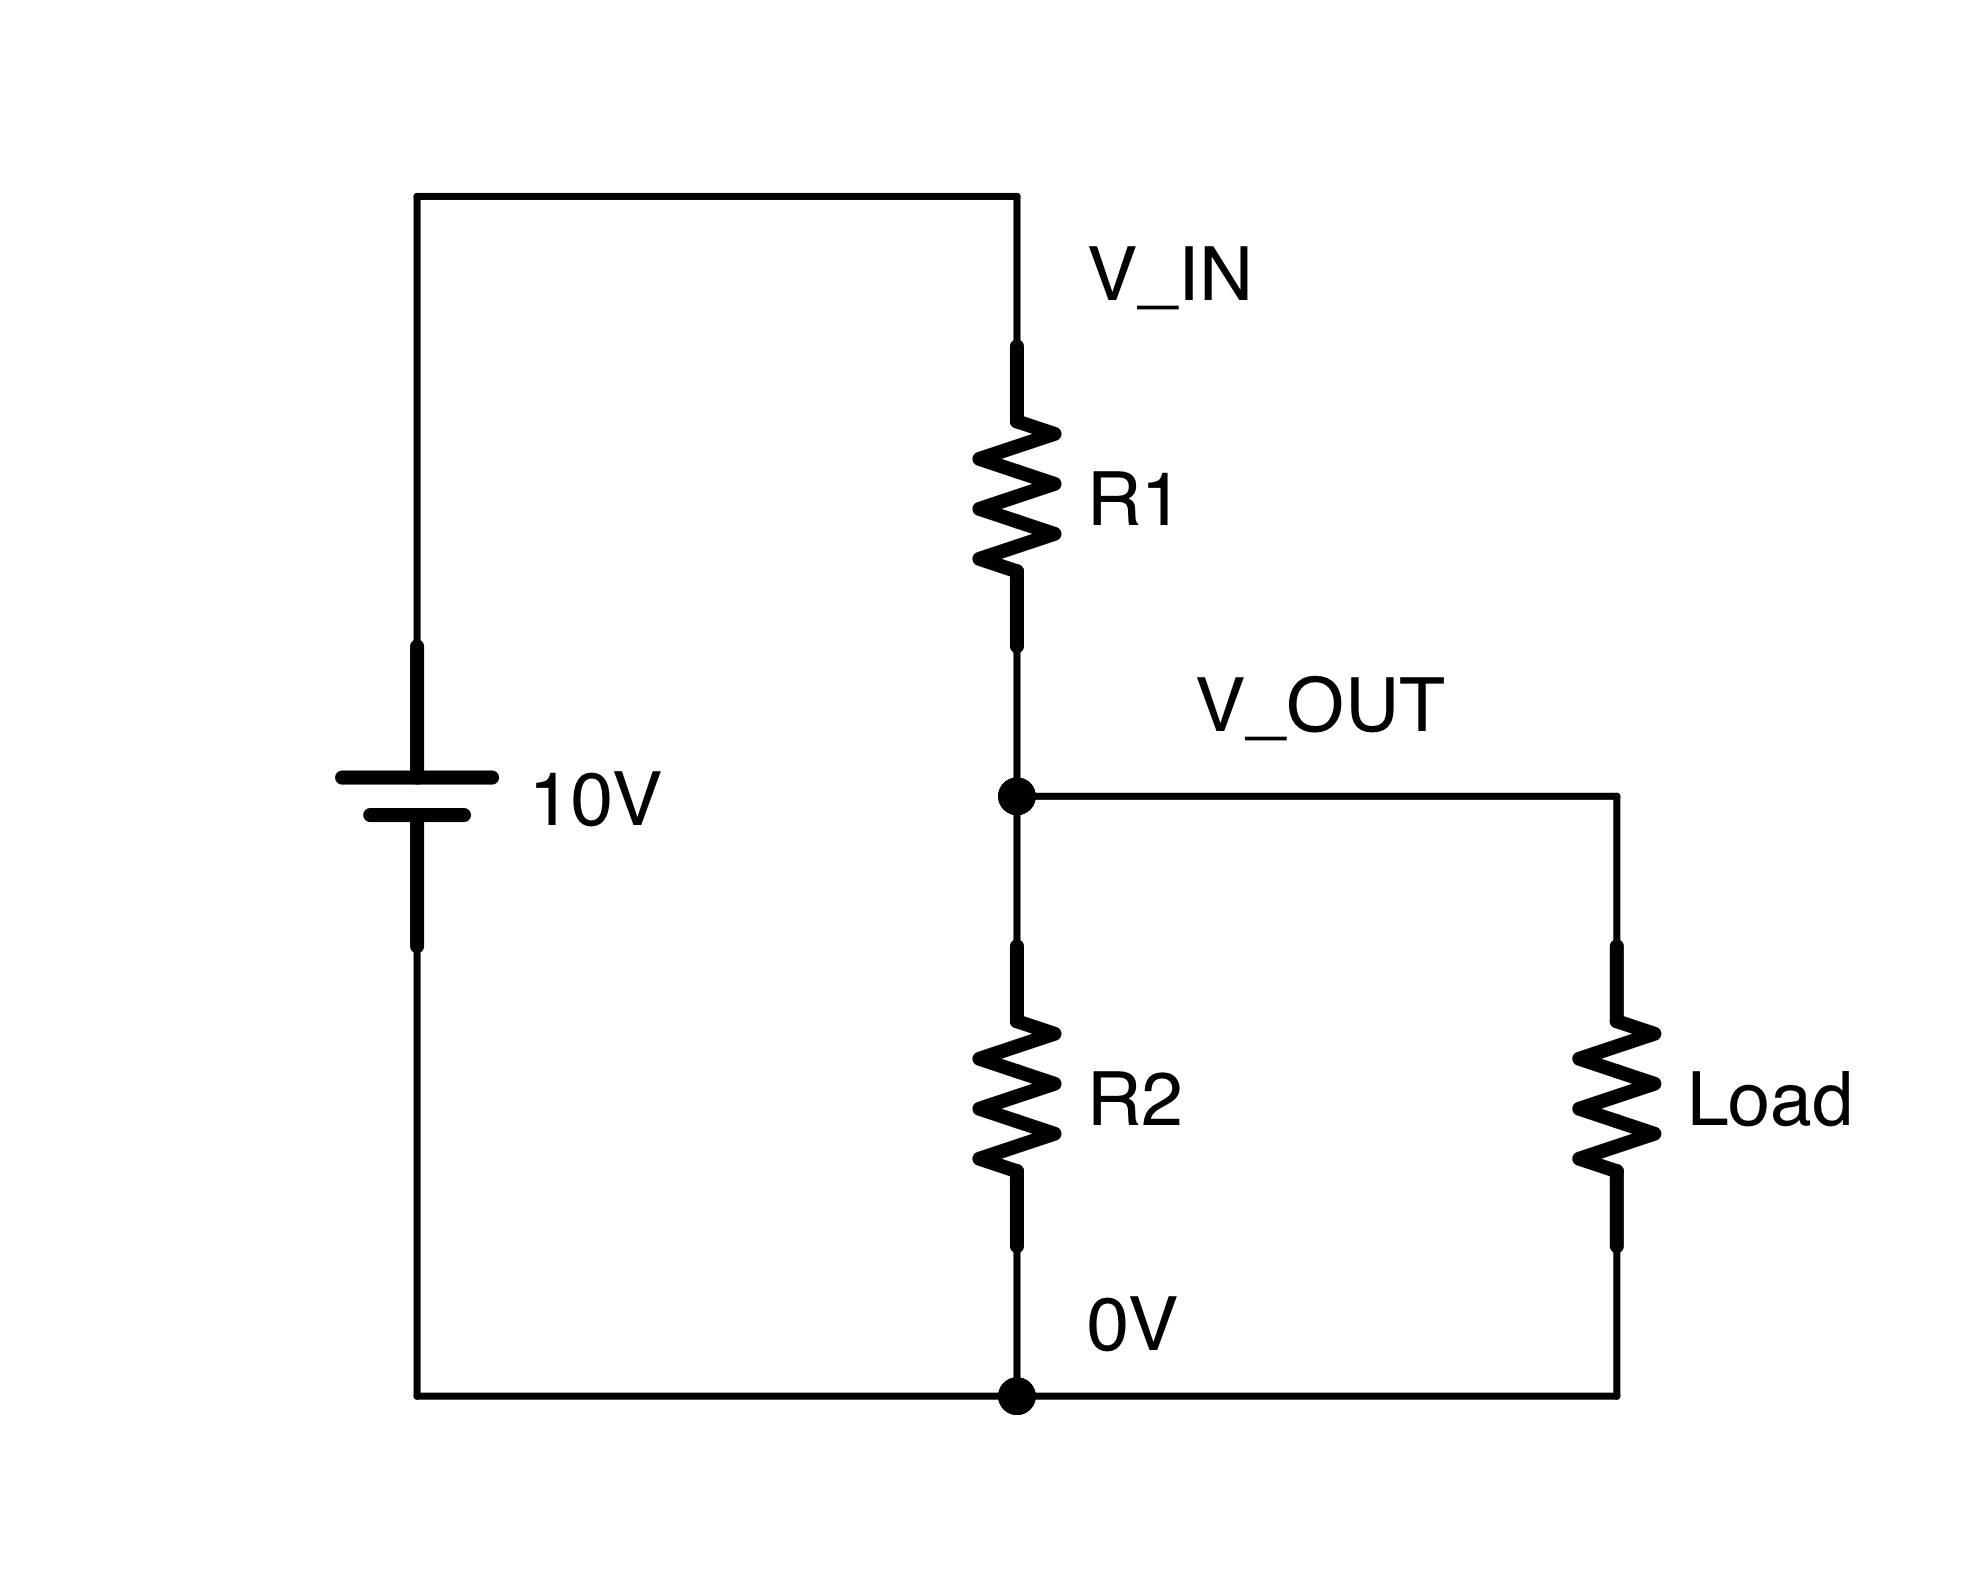
\includegraphics[width=\columnwidth]{ExVoltageDivider.png}
To achieve the required design, we need $R_1$ to be $428.57\myohm$ and $R_2$ to be $1,000\myohm$.}
\explanation{To create a voltage divider, we have to divide voltages between two resistors, with the output going out from between them.
Equation~\ref{eqVoltageDivision} shows us what the calculation looks like:
$$ V_{OUT} = V_{IN} * \frac{R_2}{R_1 + R_2} $$
Now, this equation only tells us about the ratio of the resistors, not what their specific value is.
For an equation for specific values for the resistors, we need to look at Equations~\ref{eqVDIVR2Eq} and~\ref{eqVDIVR1Eq}.
Equation~\ref{eqVDIVR2Eq} says:
\begin{align*}
R_2 &= R_L / 10 \\
    &= 10,000 / 10 \\
    &= 1,000\myohm
\end{align*}
Equation~\ref{eqVDIVR1Eq} says:
\begin{align*}
R_1 &= \frac{R_2 * (V_{IN} - V_{OUT})}{V_{OUT}} \\
    &= \frac{1,000 * (10 - 7)}{10} \\
    &= \frac{3,000}{7} \\
    &= 428.57\myohm
\end{align*}
Therefore, $R_1$ needs to be about $428.57\myohm$ and $R_2$ needs to be about $1,000\myohm$.
In reality, we would probably find a resistor that is close to $429\myohm$ even if it isn't exact.
Even a $400\myohm$ resistor would give a voltage within a few percent of the desired value.
}
\item 
\question{Given a $3\myvolt$ battery source, design a voltage divider that will output $1.5\myvolt$ to a load that has a resistance of $1\mykohm$.}
\solution{For this voltage divider, both $R_1$ and $R_2$ will be $100\myohm$.}
\explanation{Using the same equations as before, we can easily design a voltage divider. $R_2$ is determined by:
\begin{align*}
R_2 &= R_L / 10 \\
    &= 1,000 / 10 \\
    &= 100\myohm
\end{align*}
$R_1$ is determined by:
\begin{align*}
R_1 &= \frac{R_2 * (V_{IN} - V_{OUT})}{V_{OUT}} \\
    &= \frac{100 * (3 - 1.5)}{1.5} \\
    &= \frac{150}{1.5} \\
    &= 100\myohm
\end{align*}
Therefore, both $R_1$ and $R_2$ will be $100\myohm$.
}
\item 
\question{In Figure~\ref{figPullUpResistorBasic}, how much current is going through the circuit when the switch is open?  How much when it is closed?  You can assume that the LED is a red LED.}
\solution{The circuit uses $7.2\mymamp$ of current when the switch is open and $9\mymamp$ when the switch is closed.}
\explanation{When the switch is open, the current passes through \emph{both} the resistor and the LED.
Therefore, we have to account for the voltage drop of the LED itself as well as the resistance.
The starting voltage is $9\myvolt$ and a red LED will give a voltage drop of $1.8\myvolt$.
Therefore, the remaining voltage through the resistor will be $9 - 1.8 = 7.2\myvolt$.
Using Ohm's Law, we can find out the current flow:
\begin{align*}
I &= V / R \\
  &= 7.2 / 1,000 \\
  &= 0.0072\myamp = 7.2\mymamp
\end{align*}
Therefore, when the switch is open, the circuit consumes $7.2\mymamp$.
When it is closed, the current does \emph{not} flow through the LED.
The reason is that since there is a direct connection between the resistor and the ground, then the resistor \emph{must} be at a zero-volt state at the end of it.
Therefore, there is no voltage remaining to push through the LED.

Therefore, the entire $9\myvolt$ is flowing across the resistor.
This means that the calculation for Ohm's Law is as follows:
\begin{align*}
I &= V / R \\
  &= 9 / 1,000 \\
  &= 0.009 \myamp = 9\mymamp
\end{align*}
Therefore, when the switch is closed, the circuit uses $9\mymamp$ of current.
}
\item 
\question{How would you modify the circuit in Figure~\ref{figPullUpResistorBasic} to keep the maximum current in the circuit under $2\mymamp$?  Draw the full circuit out yourself.}
\solution{The full circuit should look like the below drawing:
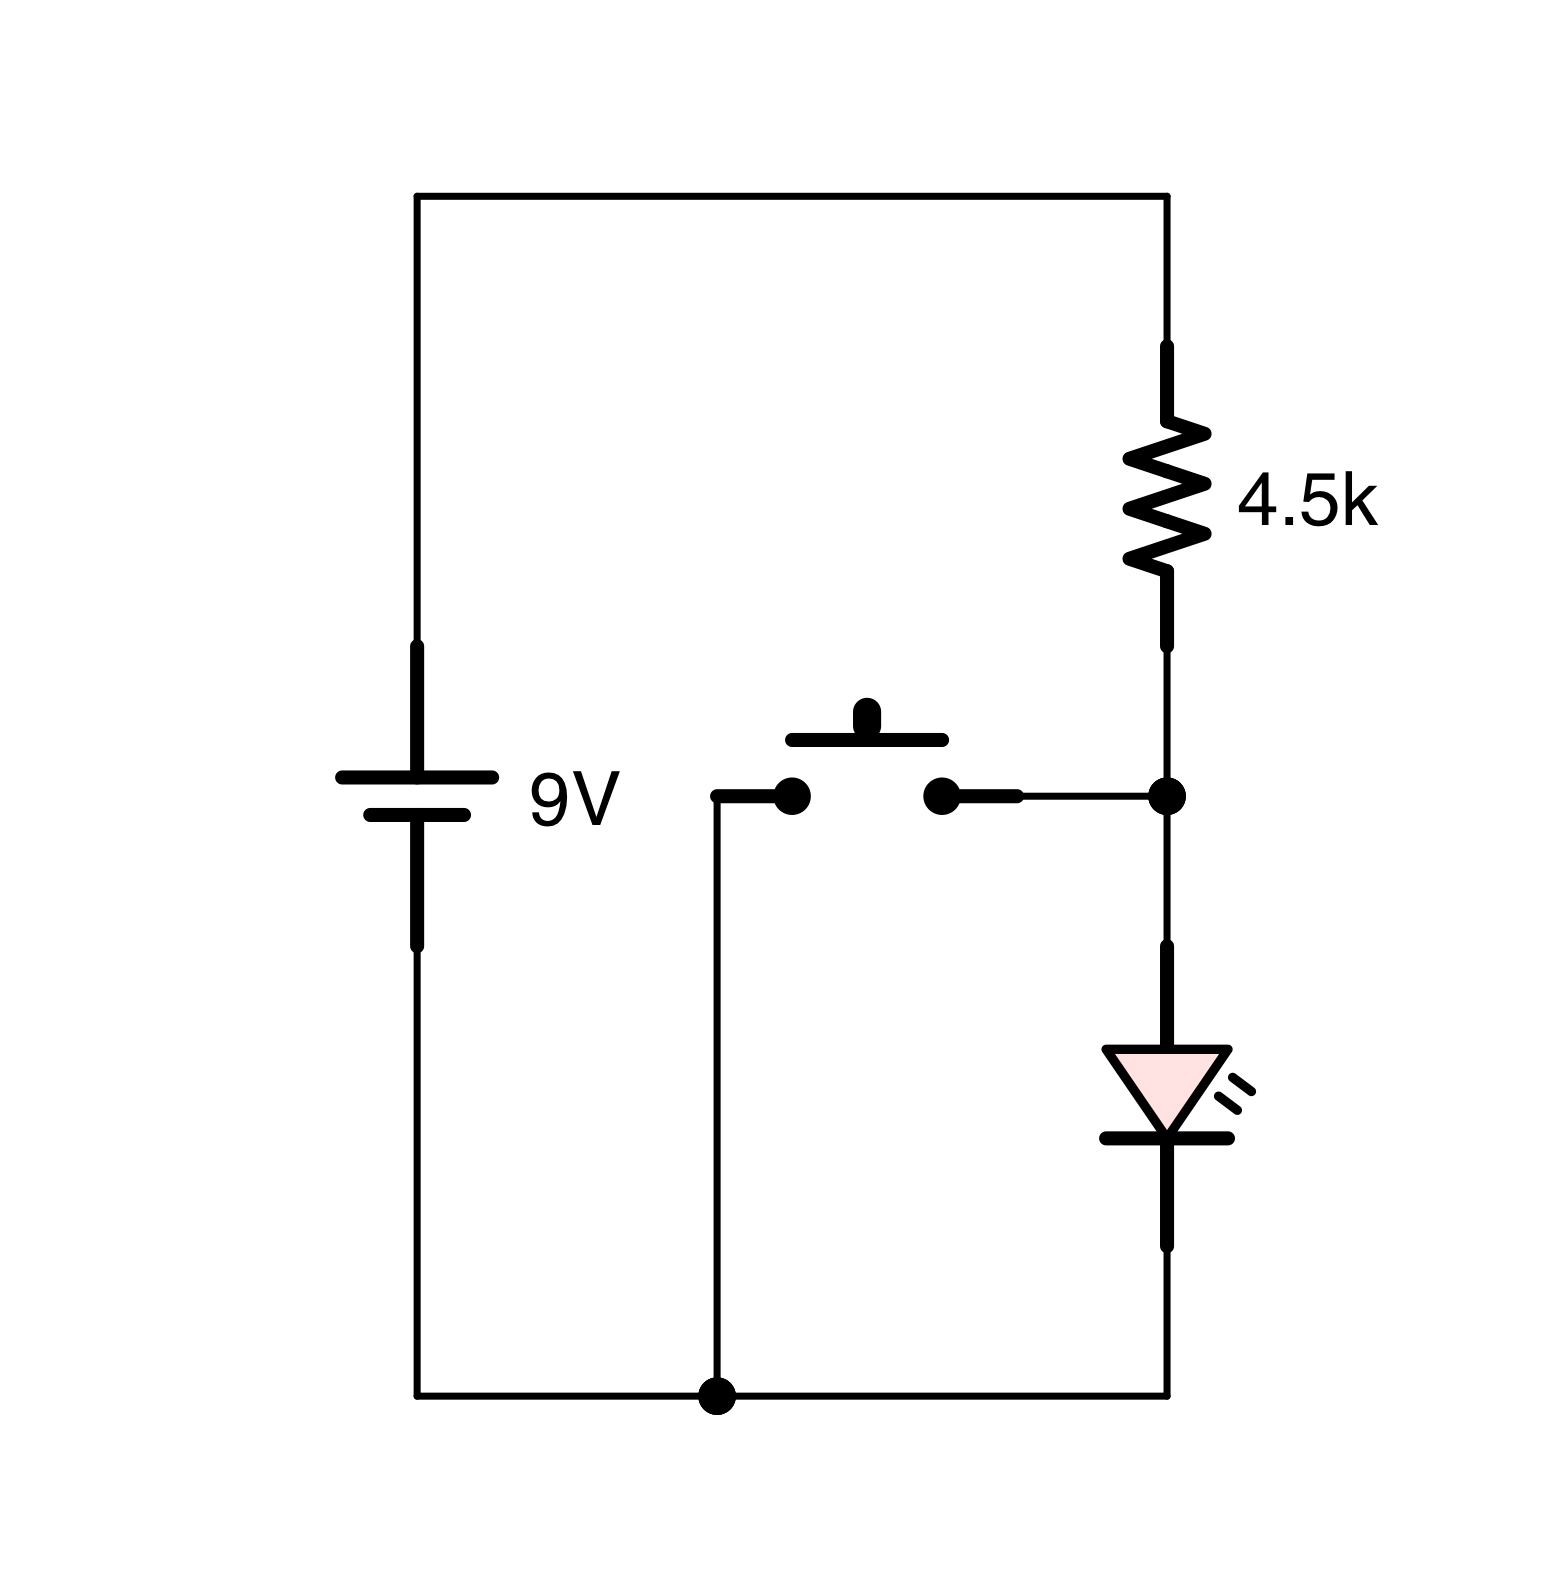
\includegraphics[width=\columnwidth]{ExPullUpResistorBasic.png}
}
\explanation{As we saw in the previous question, the circuit actually uses \emph{more} current when the switch is closed than when it is open.
Therefore, if we want to max sure the current never goes over $2\mymamp$ ($0.002\mymamp$), then we should design for that when the circuit is closed.
Therefore, using Ohm's Law, we can solve for the needed resistance like this:
\begin{align*}
R &= V / I \\
  &= 9 / 0.002 \\
  &= 4,500\myohm
\end{align*}
The drawn circuit should be identical to Figure~\ref{figPullUpResistorBasic} but with a $4,500\myohm$ resistor.
}
\item 
\question{Build the circuit you designed in the previous question.  If you do not have the right resistor values, use the closest ones you have.}
\solution{This is a project-building exercise.  The solution is correct if pushing the button turns off the light.  The one potential problem is if pushing the button creates a short circuit.  If this happens the project will get hot quickly.}
\end{enumerate}

